\chapter{Results}
\label{chap:results}

% \begin{itemize}
%     \item Average precision
%     \begin{itemize}
%         \item Main set of categories
%         \item Small set of categories
%         \item Skiing classification
%     \end{itemize}
%     \item Precision-recall curves
%     \begin{itemize}
%         \item Main set of categories
%         \item Small set of categories
%         \item Skiing classification
%     \end{itemize}
%     \item Dataset analysis
%     \begin{itemize}
%         \item Number of categories, pictures
%         \item Number of labels per picture
%         \item Top categories
%         \item Examples of Norwegian-specific categories
%         \item Examples of news-agency specific content
%     \end{itemize}
%     \item Categories tree evaluation
%     \begin{itemize}
%         \item Examples of context, double-meaning, vague labels
%         \item Examples of different children-parent relationship
%         \item Different types of labels: objects, events, state, action etc.
%         \item Granularity of categories
%     \end{itemize}
%     \item AP improvement when removing faces from sports (GTX 580 only)
%     \item Comparison of precision-recall curves of different categories
%     \item Comparison of AP for different iterations
%     \item Adam vs SGD solvers on GTX 580, small category list
%     \item Training speed comparison for Titan and GTX 580 (but CPU and SSD can also contribute)
%     \item Different split techniques
%     \item Network performance on ImageNet images* (not done yet)
% \end{itemize}


\section{Dataset analysis}
\label{sec:dataset-analysis}
Results of the initial analysis of the dataset provided by NTB are presented in this section. This analysis was the basis for the further experiments design and implementation.

NTB categories are organized in a tree structure that contains 3437 nodes, 3006 (87.5\%) of them contain at least one image, number of leaf nodes is 2804 (81.6\%), maximum depth of the tree is 6, mean depth is 3.45 with standard deviation of 0.87. There are 31 top-level categories, which are shown in Table \ref{table:top-level-categories}. This table also contains a number of descendants each top-level category has, as well as a total number of pictures that belong to this category subtree. Each image can belong to zero or more categories, meaning that categories were not designed to be mutually exclusive on any level of the categories tree. Top 20 categories with the most pictures in them are shown on the Figure \ref{fig:top-cats-distribution}.  Provided NTB dataset contains 912324 of images, 805946 (88\%) of them have at least one label, therefore belong at least to one category. The whole category tree is too big to visualize it in any way, however, the most important highlights and insights are provided further in this section.

\begin{table}[h!]
    \centering
    \csvautotabular[respect sharp]{tables/top-level-categories.csv}
    \caption{Top Level categories with total number of descendants and images}
    \label{table:top-level-categories}
\end{table}

\begin{figure}[h!]
    \centering
    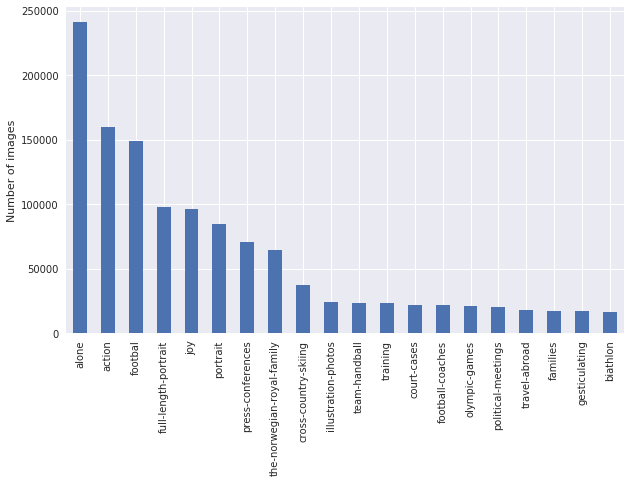
\includegraphics[width=0.9\textwidth]{top-cats-distribution}
    \caption{Distribution of images in top 20 categories}
    \label{fig:top-cats-distribution}
\end{figure}

From both Table \ref{table:top-level-categories} as well as Figure \ref{fig:top-cats-distribution} it is possible to see that the provided dataset is focused on sports, politics and finance topics, which is expected since NTB is a Norwegian news content providing company. Further analysis also shows that many categories are specific to Norway, for example \textit{norwegian-royal-family}, \textit{cross-country-skiing}, \textit{the-king's-throne-speech}, \textit{the-parliament-building}, \textit{stave-churches}, \textit{norwegian-national-costumes} etc. The category types are also very diverse. For example there are categories which represent simple objects (\textit{tv-sets}, \textit{cars}, \textit{doors}), abstractions (\textit{communism}, \textit{neo-nazism}), group of people (\textit{policemen}, \textit{politicians}, \textit{christians}), holidays (\textit{christmas}, \textit{national-days}), relationships (\textit{grandchildren}, \textit{daughters}), sports (\textit{skiing}, \textit{football}), actions (\textit{handshake}, \textit{document-signing}) etc.

Figure \ref{fig:num-labels} illustrate the distribution of the number of labels per one image in the dataset. Most of the images have from two to four labels associated with them. This fact together with the non-mutual exclusive set of categories, as well as the real-world nature of the images (which potentially are more crowded), makes a multi-label classification system more suitable for this dataset than a single-label. There is a label \textit{alone} in the NTB set of categories that is used to identify images which contain a single object. This label should not be confused with a single-label case of classification since even if there is only one object on the picture, in the multi-label case it can belong to several categories which describe this object. For example, even though figures \ref{fig:without-sign-of-triumph} and \ref{fig:with-sign-of-triumph} both contain label \textit{alone}, they both also contain number of other labels that describe these pictures in different dimensions (kind of sport, gender, emotions etc).

\begin{figure}[h!]
    \centering
    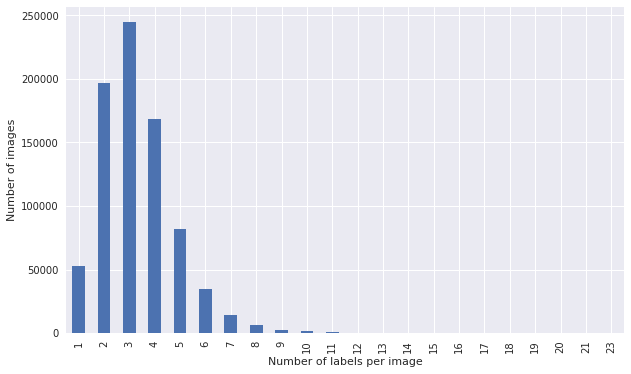
\includegraphics[width=0.9\textwidth]{num-labels}
    \caption{Number of labels per one image distribution}
    \label{fig:num-labels}
\end{figure}

Analysis of the categories tree, as well as example images from different categories, revealed some issues connected with the dataset described further.

\paragraph{Mistakes and not visible entities}
The dataset contain different classification mistakes like missing or extra labels on the picture. In many cases labeled object on the picture is not located in the center or even clearly visible. For example, picture labeled as \textit{blueberries} is shown on Figure \ref{fig:image-blueberries}. No blueberries are visible on this image, the main entity visualized on the picture is a person. However, the image is not even labeled with the tag \textit{person}. 

\begin{figure}[h]
    \centering
    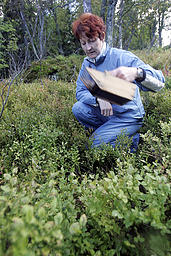
\includegraphics[width=0.4\textwidth]{images/sp616962}
    \caption[Example picture from the \textit{blueberries} category]{\textit{blueberries}, \textit{berries}, \textit{autumn}, \textit{illustration-photos}. Photo by Terje Bendiksby~/~Scanpix}
    \label{fig:image-blueberries}
\end{figure}

\paragraph{Background objects}
In some cases labeled object is visible, but not located in the main scene of the picture or is part of the background. For example, on Figure \ref{fig:image-flowers} two pictures classified as \textit{flowers} are shown, however while on both pictures it is possible to see flowers, but they are either surrouned by other objects on the scene or are on the side of it.

\begin{figure}[ht!]
    \centering
    \begin{subfigure}[a]{0.45\textwidth}
        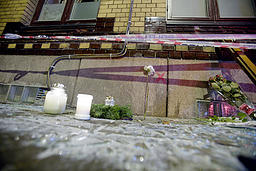
\includegraphics[width=\textwidth]{images/flowers/sx907808}
        \caption{\textit{flowers}, \textit{candles}, \textit{apartment-houses-in-the-city}, \textit{fires}, \textit{death}, \textit{house-fires}, \textit{crime-scenes}. Photo by Stian Lysberg Solum~/~Scanpix}
    \end{subfigure}
    ~
    \begin{subfigure}[a]{0.45\textwidth}
        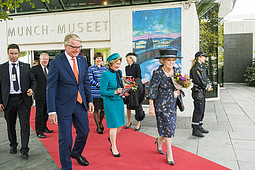
\includegraphics[width=\textwidth]{images/flowers/ta550898}
        \caption{\textit{red-carpet}, \textit{flowers}, \textit{the-norwegian-royal-family}, \textit{policemen}, \textit{full-length-portrait}, \textit{art-exhibitions}, \textit{hats}, \textit{the-dutch-royal-family}, \textit{opening-ceremonies}. Photo by Fredrik Varfjell~/~Scanpix}
    \end{subfigure}
    \caption{Example pictures from \textit{flowers} category}
    \label{fig:image-flowers}
\end{figure}


\paragraph{Not consistent labels}
Some labels are not consistent across the whole dataset. For example, \textit{sign-of-triumph} label is applied on images that have person with two hands raised up. However, often this label is missing on images and only label \textit{joy} is applied. This issue is illustrated on Figure \ref{fig:sign-of-triumph-example}, where from two visually similar images only one has \textit{sign-of-triumph} label.

\begin{figure}[ht]
    \centering
    \begin{subfigure}[a]{0.3\textwidth}
        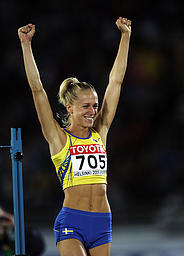
\includegraphics[width=\textwidth]{images/sp8718f2}
        \caption{\textit{alone}, \textit{athletics}, \textit{high-jump}, \textit{women}, \textit{sign-of-triumph}, \textit{joy}. Photo by Cornelius Poppe~/~Scanpix}
        \label{fig:with-sign-of-triumph}
    \end{subfigure}
    ~
    \begin{subfigure}[a]{0.3\textwidth}
        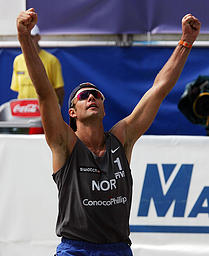
\includegraphics[width=\textwidth]{images/sp525daa}
        \caption{\textit{alone}, \textit{beach-volleyball}, \textit{action}, \textit{joy}. Photo by Alf Ove Hansen~/~Scanpix}
        \label{fig:without-sign-of-triumph}
    \end{subfigure}
    \caption[Example of two similar images and with different labels]{Example of two similar images and with different labels. Only one image belongs to \textit{sign-of-triumph} category}
    \label{fig:sign-of-triumph-example}
\end{figure}

\paragraph{Different purpose of labels}
Labels in the NTB dataset can have a different purpose. Most of the labels define some entity or action that is presented in the picture. However, some labels are designed to be a modification of other labels. For example, label \textit{action} was designed to be used together with any sports category like \textit{football} to get football players in action. Mentioned earlier label \textit{alone} serves to identify images withing particular category with only one object illustrated on them. This inconsistency can potentially influence resulting classification system performance.

\paragraph{Contextual categories}
There are many contextual categories, where visual information is not enough to determine if image should belong to the category and additional context information is necessary. Example of such categories: \textit{second-hand-cloth}, \textit{used-cars}, \textit{counterfeit-money}, \textit{finance-debates}. More issues discovered during category tree evaluation are presented in Section \ref{sec:tree-eval}.

\paragraph{Contextual images}
There are many images which have an assigned category that can not be derived only from the image itself and more contextual information is needed. For example, picture that is part of the category \textit{politicians} as well as \textit{fishfarming} and \textit{fisheries-industry} is shown on Figure \ref{fig:politician-fish}. While the first category can potentially be automatically derived using face-recognition approach, the second and the third categories are fully contextual. In order to assign these labels to the picture, the system needs more additional information such as when and where the picture was taken as well as what was discussed in this place and time. Another example is press-conference or portrait pictures that are part of some sports category. From 151533 images of football, 151533 (10.4\%) belong to the \textit{coaches}, \textit{press-conferences} or \textit{portrait} categories as well.

\paragraph{Similar images}
Due to real-world nature of the used dataset, there are groups of pictures that were taken from one event. As a result, some images are visually very similar to each other. This issue can arise during the split of the dataset on training, validation and test parts. If two similar images will end up in two different sets it can potentially influence the reported precision of the system.

\begin{figure}[h]
    \centering
    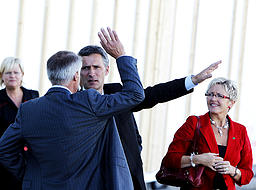
\includegraphics[width=0.6\textwidth]{images/sy253353}
    \caption[Example of contextual labeled images]{\textit{politicians}, \textit{fishfarming}, \textit{fisheries-industry}, \textit{travel-in-norway}. Photo by Gorm Kallestad / Scanpix}
    \label{fig:politician-fish}
\end{figure}

The reason for all of the mentioned issues can potentially be that the dataset, as well as its categories tree, were not designed for future automated classification system training. They, however, can influence negatively such system performance. Further sections of this thesis will try to address and discuss these discovered issues from the perspective of a creation of multi-label image classification system.

The size and uniqueness of the NTB dataset make it perfect subject of the research on real-world datasets that were not originally designed for automatic classification training and can be used to find possible solutions for presented issues that can also exist in other datasets of this kind. Broad, diverse and unique set of NTB categories also eliminates the possibility to direct use of the systems trained on a more standard set of categories like ImageNet. Therefore, training system on a new set of categories should be performed.

% Pictures total:  912324
% With tags:  805946
% Multiple tags: 93.5%

\section{Trial experiment}
As it was mentioned earlier, a set of trial experiments were performed for multiple reasons, including to get a better understanding of the neural networks potential when trained on the available dataset, to test training and testing implementations, and to get insights on which hyperparameters works better for this purpose.

All experiments performed during the trial part of the research were made on the set of categories, which selection was described in Section \ref{sec:trial-cat-selection}. Results of the best network trained from the set of trial experiments are presented in the first section. The next section shows performance improvement achieved by filtering out the part of contextual images from the dataset. A comparison of two solver algorithms is shown in the third section, while the comparison of the training speed using two different solutions for data layer of the neural network is presented in the last section.

As it was described in Section \ref{sec:trial-dataset-prep} all trial experiments, except the comparison of performance with and without contextual images removed, were performed on different, randomly generated subsets of initial dataset. Therefore a direct comparison of the results from different experiments might not be precise enough. There can potentially be some variations in the results due to differences in the datasets. However, the results can give indications of whether one method of training is significantly better than the other.

\subsection{Classification performance}
    Results presented in this section were obtained from the network trained using the Adam solver algorithm for 1000 iterations. The image dataset was additionally filtered from contextual images, this is further described in the next section.
    
    Training and validation loss curves are shown on Figure \ref{fig:trial-training-curve}. It is clearly visible that both losses go down, which is expected. This is also a sign that overfitting is not taking place at this level of iterations
    
    \begin{figure}[H]
        \centering
        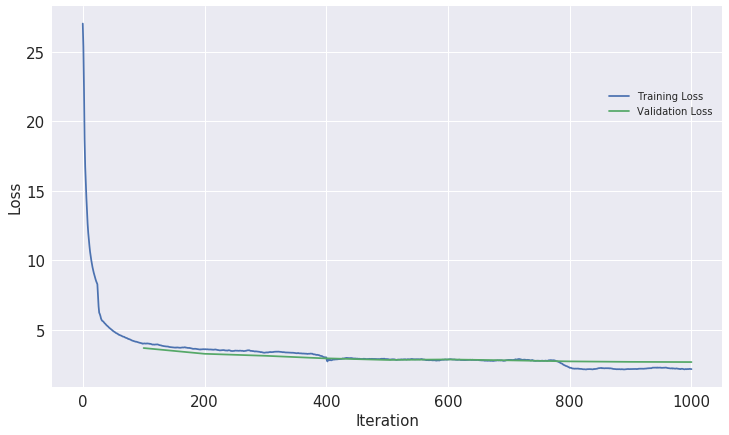
\includegraphics[width=\textwidth]{trial/adam_rmportraits/training_curve}
        \caption{Training and validation loss curve during trial experiment}
        \label{fig:trial-training-curve}
    \end{figure}
    
    The resulting average precision for each category is shown on Figure \ref{fig:trial-average-precision}. 10 (25.6\%) out of 39 categories have an average precision of more than 80\%. All these categories, except \textit{cars} and \textit{boats} are belong to sports. 29 (74.4\%) categories have an AP of more than 60\%.

    \begin{figure}[H]
        \centering
        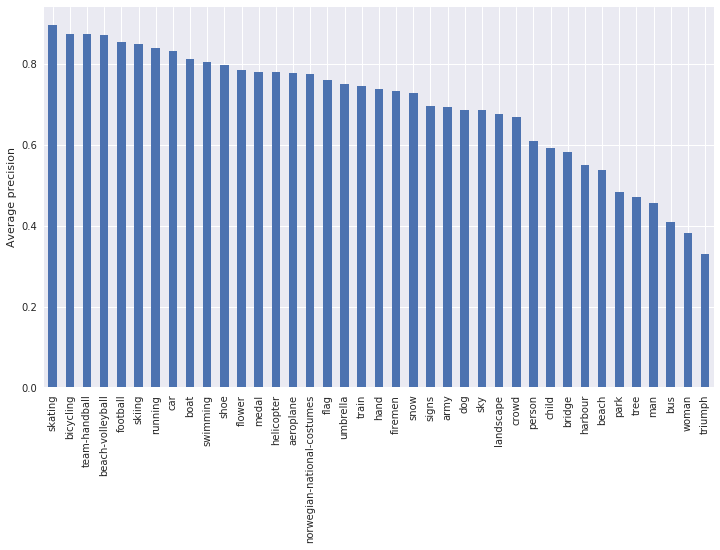
\includegraphics[width=\textwidth]{trial/adam_rmportraits/average_precision}
        \caption{Average precision results for trial experiment}
        \label{fig:trial-average-precision}
    \end{figure}
    
    The relationship between the average precision for each category and the sample size used for training is shown on Figure \ref{fig:trial-average-precision-vs-size}. The chart shows a non-linear dependency between the two values. The categories with the biggest sample sizes have the highest average precision values, however high values of average precision is also represented in categories with smaller sample sizes. Some of the categories with high sample sizes have a lower value of average precision. The potential reason for this can be that there are challenges connected with the category itself when it comes to automatic classification. The same reason could apply to the fact that categories with similar values of sample sizes have very different average precision (for example \textit{bus} and \textit{shoe}).
    
    \begin{figure}[H]
        \centering
        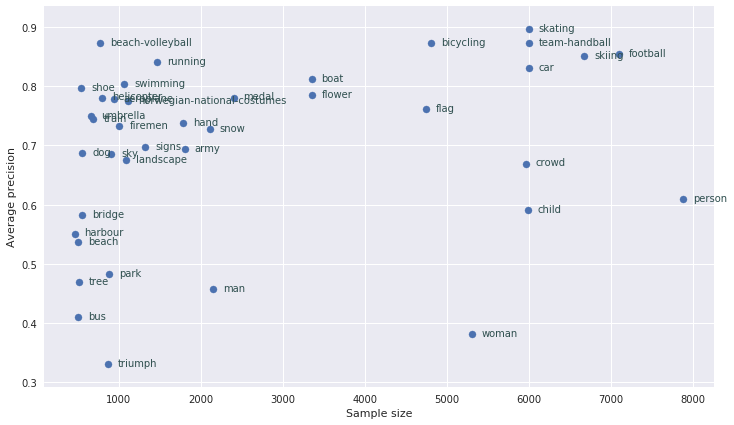
\includegraphics[width=\textwidth]{trial/adam_rmportraits/average_precision_vs_size}
        \caption{Average precision vs category sample size used for training}
        \label{fig:trial-average-precision-vs-size}
    \end{figure}
    
    Figure \ref{fig:trial-400-vs-1000} shows a comparison of average precision values for different iterations. As expected, average precision increases with further training. An additional observation is that further training appears to have a bigger effect on categories with lower values of average precision, compared with categories with higher values which got a lower increase in the precision. Therefore the difference between higher and lower categories decreases in line with the number of passed iterations.
    
    \begin{figure}[H]
        \centering
        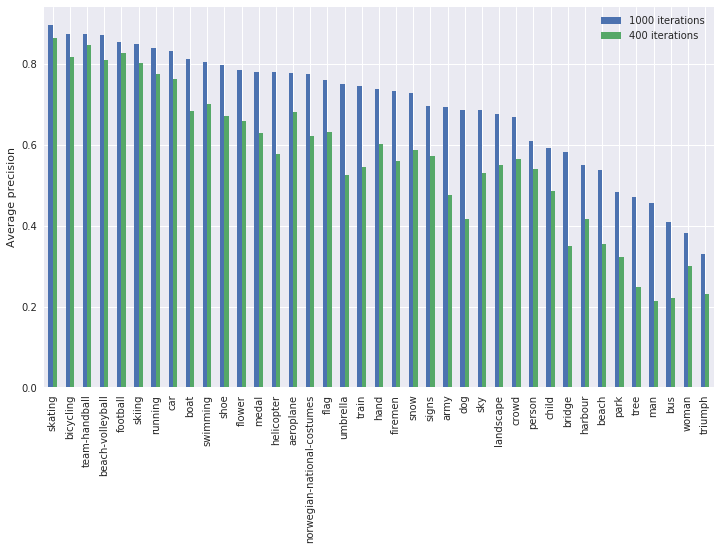
\includegraphics[width=\textwidth]{trial/adam_rmportraits/400_vs_1000_ap}
        \caption{Comparison of the average precision for network on 400 and 1000 iterations during trial experiment}
        \label{fig:trial-400-vs-1000}
    \end{figure}
    
    As it was described in Section \ref{sec:trial-testing}, average precision is calculated based on the precision-recall curve for each category. An example such curve (for the best category of \textit{skating}) is shown on Figure \ref{fig:trial-precision-recall-skating}. It shows that around 80\% of the \textit{skating} images can be found with almost 100\% of precision. Figure \ref{fig:trial-precision-recall-woman} shows the precision-recall curve for one of the lowest categories (\textit{woman}). In comparison to the previous chart, it is clearly visible that the precision drops much faster with higher values of recall.
    
    \begin{figure}[H]
    \centering
    \begin{subfigure}[a]{0.9\textwidth}
        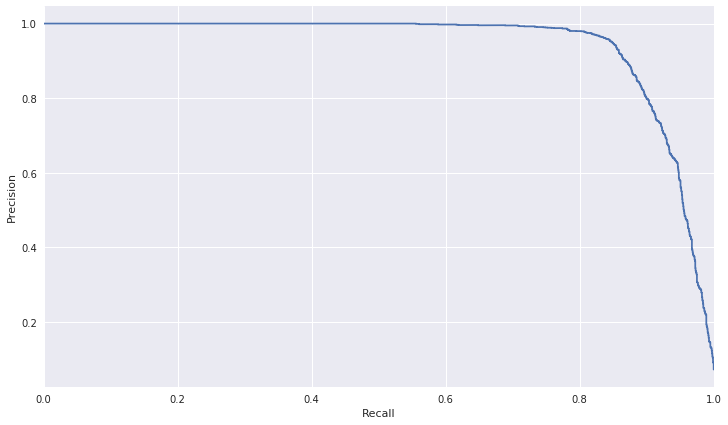
\includegraphics[width=\textwidth]{trial/adam_rmportraits/recall_precision_skating}
        \caption{Precision-recall curve for \textit{skating} category}
        \label{fig:trial-precision-recall-skating}
    \end{subfigure}
    \\
    \begin{subfigure}[a]{0.9\textwidth}
        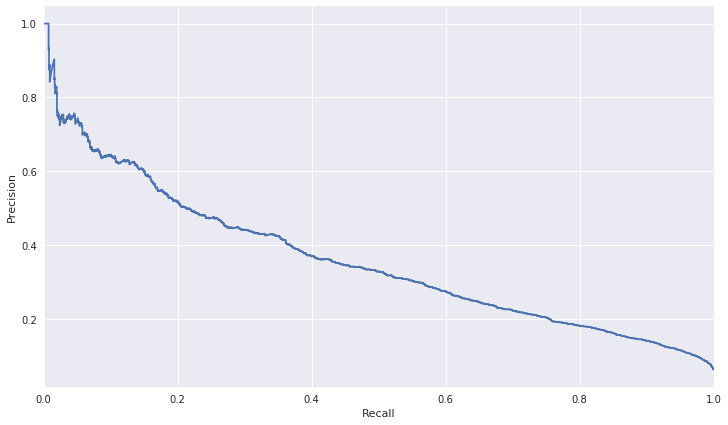
\includegraphics[width=\textwidth]{trial/adam_rmportraits/recall_precision_woman}
        \caption{Precision-recall curve for \textit{woman} category}
        \label{fig:trial-precision-recall-woman}
    \end{subfigure}
    \caption{Precision-recall curves for one of the best and worst categories}
    \end{figure}
    

\subsection{Context improvements}
    In order to show the potential improvement that can be achieved by filtering contextual images from the dataset, separate experiment was performed. As it was mentioned in Section \ref{sec:trial-cat-selection}, images labeled as \textit{portrait}, \textit{press-conferences} and \textit{coaches} were removed from all categories except \textit{woman}, \textit{umbrella}, \textit{hand}, \textit{person}, \textit{norwegian-national-costumes}, \textit{child}, \textit{medal}, \textit{triumph}, \textit{man}. The goal was to remove portraits of persons (such as portraits of sportsmen or their coaches) and press-conference pictures since it was considered that in order to classify such images in certain categories (like \textit{football} or \textit{skating}) either additional information or a face-recognition system is needed.
    
    The first network was trained for 1000 iterations on a randomly generated dataset (as described in Section \ref{sec:trial-cat-selection}), then contextual images were removed from the specified categories and a new network was trained for 1000 iterations on the filtered dataset. Results from both experiments are shown on Figure \ref{fig:trial-allpics-vs-rmportraits}.
    
    \begin{figure}[H]
        \centering
        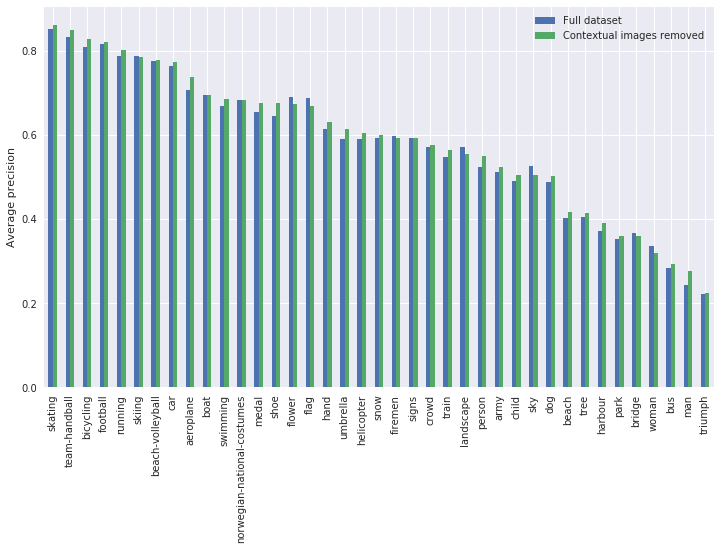
\includegraphics[width=\textwidth]{trial/adam_allpics_vs_rmportraits_ap}
        \caption{Comparison of average precision for network on 400 and 1000 iterations during trial experiment}
        \label{fig:trial-allpics-vs-rmportraits}
    \end{figure}
    
    28 (71.8\%) out of 39 categories got improvement in their average precision values. Including 7 categories from those which were skipped in the filtering process and had exactly the same dataset. 6 of the categories reduced their average preformance. One explanation of these results can be that in the used neural network implementation output probabilities from the final fully-connected layer are not fully independent from each other since they can depend on the same features from the earlier layers. Features learned on images from one category can also be used to produce probabilities for other categories, therefore changes in a sample for one category can influence end classification of the other.
    
    % TODO: MAYBE TO INCLUDE MEAN
    
    Results give an indication that end system classification performance can be potentially improved by removing fully contextual images from the dataset. Section \ref{sec:real-world-dataset-challenges} contains further discussion on obtained results.

    
\subsection{Adam vs SGD}
    An additional experiment was conducted in order to test which solver algorithm works better for the purpose of the research. As it was described in Section \ref{sec:trial-training} two widely used algorithms were compared: Adam and Stochastic Gradient Descent (SGD). Two separate networks were trained for 1000 iterations with corresponding algorithm applied. Resulting average precision for both networks is shown on Figure \ref{fig:trial-sgd-vs-adam}.

    \begin{figure}[H]
        \centering
        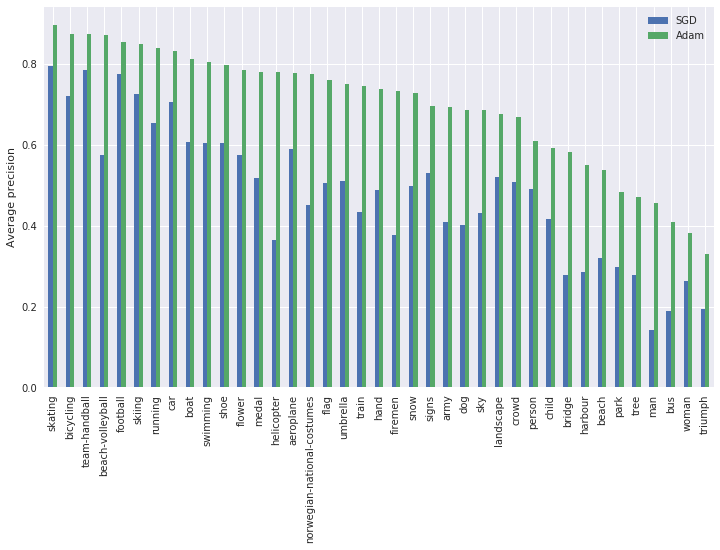
\includegraphics[width=\textwidth]{trial/adam_vs_sgd_rmportraits_ap}
        \caption{Comparison of average precision for network trained using SGD and Adam solver algorithms}
        \label{fig:trial-sgd-vs-adam}
    \end{figure}
    
    Due to a significantly better average precision resulting from the training for the same amount of time, Adam solver was used in all further experiments.
    
    
\subsection{LMDB vs Python DataLayer}
    % ASK IF IT SHOULD BE HERE OR ONLY IN METHODS
    All trial experiments were performed on a relatively small selection of categories and a total number of images. This allowed the author to perform experiments in a short period of time. During main experiments, however, a much broader set of categories was employed. The total number of images used in the training and testing process was therefore also increased. This could impact the overall training time of the system. Therefore it was decided to investigate on possible optimizations of the current system implementation. Since all computational layers in the system pipeline were already leveraging GPU, the bottleneck of the whole system was seemingly the first Python data layer. The Python data layer was used in the trial set of experiments due to its flexibility. For the main experiments, however, flexibility was considered less important and speed was a priority because of the increased dataset size. The Caffe framework supports other, more optimized ways to deliver image data inside the network. As it was described in Section \ref{sec:trial-training}, Lightning Memory-Mapped Database (LMDB) was chosen as an alternative source of image data.
    
    An additional experiment was therefore performed in order to get insights on the potential speedup of the system training process while using this database. As it was mentioned earlier, due to the limited interface provided by the Caffe LMDB module, a single-label classification system was trained. Specifically, the skiing category was selected due to the mutually exclusive property of its descendants withing the NTB dataset. Two networks were trained during this experiment: one using Python layer as an image data source, and one that was loading images from the prepared LMDB file.
    
    Based on the reported numbers provided by the Caffe framework, an average value of 0.1045 iterations per seconds was achieved by the network that used a Python data layer, while the other network was operating on 0.5381 iterations per second. Therefore, by using LMDB file as an image data source the system achieved more than 5 times speedup during the training process. 
    
    The resulting average precision of the skiing type classification is shown on Figure \ref{fig:trial-skiing-ap}.
    
    \begin{figure}[H]
        \centering
        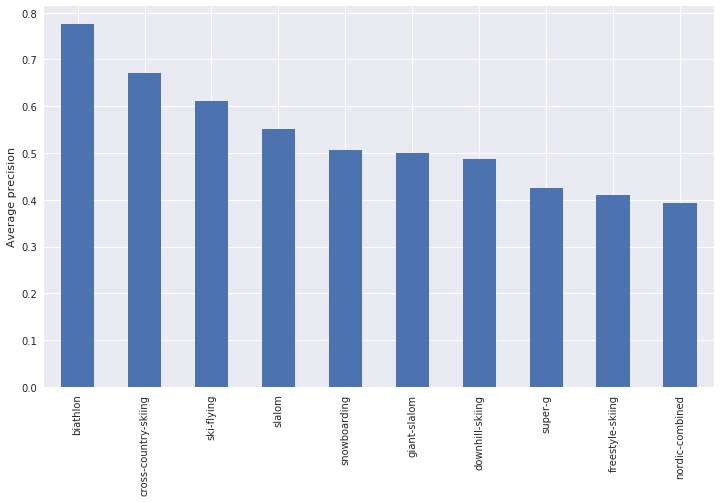
\includegraphics[width=\textwidth]{trial/skiing_ap}
        \caption{Average precision result of the skiing type classification}
        \label{fig:trial-skiing-ap}
    \end{figure}
    

\section{Main experiment}
All lessons learned during the trial set of experiments were applied to perform experiments on a more broad set of categories. The goal of this part of the research was to use as much of dataset provided by NTB as possible. The first section gives insights on how initial NTB categories tree was changed and improved for multi-label classification system training. Comparison of the two dataset splitting methods is shown in the second section. The results of the two trained classification systems are presented in the last section.

\subsection{Category tree evaluation and improvement}
    \label{sec:tree-eval}
    As it was described earlier, NTB provided the author with categories organized in a tree structure. Images in the dataset can be labeled parent and child categories. However, both neural network implementations that were adapted to be used in this study, as well as other ones available in the ModelZoo \cite{CaffeModelZoo} collection, were designed to be trained on a flat set of categories, without any utilization of the information about the relationship between them. Therefore, the first observation was that until existing neural networks will be able to use this information during the training process, any categories hierarchical structure had to be transformed into a flat representation. Several automatic approaches were tested, all of which failed due to different reasons described further.
    
    The first attempt of automatic approach was to include all categories without any modifications. The problem with this solution is that in many cases when there was subclass relationship between parent and child categories (for example \textit{trees} and \textit{oak-trees}) only part of the images from the child category was also labeled with the parent (only part of \textit{oak-trees} were labeled as \textit{trees}). This inconsistency in the way images are labeled had to be addressed since in another case in could influence the overall performance of the system. Therefore the second approach was to automatically include into the parent category all images of its descendants. It was discovered, however, that many relationships between categories were not of the subclass type. For example, \textit{trees} $\rightarrow$ \textit{leaves} (part-of relationship type), \textit{football} $\rightarrow$ \textit{football-pitches}, \textit{war} $\rightarrow$ \textit{resistance} and \textit{banks} $\rightarrow$ \textit{atms}. The main issue is that it is hard for an automatic system to know which type of relationship the terms have. The third automatic solution was to use only leaves of the tree and remove all other categories. While it would fix previous issues, this approach would require removing a big portion of metadata information that otherwise could be utilized by the system. One example of this would be to remove category of \textit{football} and to keep only its descendants: \textit{football-pitches}, \textit{footballs}, \textit{beach-soccer} and \textit{penalty-kicks}. However, the \textit{football} category contain 150016 images, while all its descendants combined have only 807 images. It was also discovered that it was not possible to make a decision on if parent category should be included or not based only on a number of pictures in the category itself and its children due to inconsistency in the relationship types mentioned earlier. In addition to mentioned problems, the general issue with the automatic approach to category tree transformation is that many categories are not suitable for training of a classification system. The following issues with categories were discovered through the tree evaluation:
    
    \begin{itemize}
        \item Some categories were abstract terms like \textit{genocide}, \textit{love}, \textit{future} or \textit{daily-life}.
        \item In some cases category name could have double meaning. For example, \textit{direction} can mean the direction sign, or person pointing direction.
        \item Category names can be fully contextual, which mean that in order to classify the image into this category it is necessary to have additional information about it. Examples of such categories: \textit{grandfathers}, \textit{second-hand-cloth}, \textit{used-cars}, \textit{counterfeit-money}, \textit{war-criminals}. An additional discovery was that some categories were classified as contextual only with the knowledge about specific nature of the dataset. For example, categories \textit{prisoners} and \textit{prisons} were not included because pictures of Norwegian prisoners and prisons can hardly be distinguished from other images due to the special properties of Norwegian penology system.
        \item Category name was a combined term. Examples: \textit{childhood-and-youth-pictures}, \textit{moos-and-lichen}, \textit{fires-in-trains}. The last example category also shows that is some cases one category represented connection of other ones, \textit{trains} and \textit{fire} in this case. Multi-label classification system can potentially discover such connections automatically by assigning both labels to the image.
        \item Some categories were representing a combined action. Examples: \textit{thriatlon} (different types of sports), \textit{nordic-combined} (different types of skiing). It can be hard to classify such categories since there are many pictures with only one type of sport visualized at the same time. The category \textit{biathlon} is an exception since in this case sportsman's gun can be an indicator of pictures from this kind of sport. \textit{biathlon} category is also a good example of why manual selection of categories have be performed rather than automatic one.
    \end{itemize}
    
    Due to all reasons described above the decision on which category to include had to be made for each case separately. Therefore all 3437 NTB categories were examined manually in order to create a new tree of categories, adapted for multi-label classification training. For reasons described earlier it was decided to use leaves of the categories tree where is was possible with a few exceptions in order to get maximum granularity of the end classification. The overall category tree transformation method designed and used in this research is described in Section \ref{sec:main-cat-selection}.
    
    The final categories set contained 1507 categories, from which 1440 (95.55\%) were directly copied from the NTB dataset without any changes. The rest 67 categories were created by merging images from other categories. 23 (34.33\%) of them were extended with images of all their descendants (for example \textit{dogs}, \textit{mushrooms}, \textit{shoes}), while the rest of them were combined from a selected set of subcategories. An example of such selection is created category \textit{trees} that combined images of all tree types, but did not include images of such children categories like \textit{leaves} or \textit{branches}. Another example is category \textit{person} that was created by merging images labeled with original \textit{persons} NTB category as well as such categories as \textit{women}, \textit{men}, and even such context categories as \textit{grandmothers} and \textit{sons} which were not included in the final selection as a separate categories.
    
    As it was described in Section \ref{sec:main-dataset-prep} due to difficulties in dataset splitting connected with cross-categories connections in multi-label case, only categories with a minimal number of 50 images were included in the final set. Therefore from 1507 selected categories, only 663 were used for actual training.

\subsection{Dataset split method}
    \label{sec:split-comparison}
    As it was described in methods chapter, different dataset splitting algorithms were used during trial and main experiments. Comparison of the dataset distribution across training, validation and test sets of both methods is shown on Figure \ref{fig:main-split-distribution}. Horizontal axes of both histograms show a percentage of included images from the original image dataset of the particular category, while vertical axes represent an amount of categories with this percentage. The histogram of the new splitting method shown on Figure \ref{fig:main-split-distribution-main} follows the curve of normal distribution for all sets, with the mean values of the desired ratio (60\% for the training set, 20\% for both validation and test sets). Therefore most of the categories in all three sets contain around the target amount of images with a smaller number of other categories below and above target values. Due to another, prioritized, method used in the trial experiments, distribution on Figure \ref{fig:main-split-distribution-trial} has another shape. Validation and test sets had higher priority than training set, therefore both of them have higher mean value than the target 20\%. Therefore most of the categories from validation and test sets contain more than 20\% of images from the original dataset. Because of that, training set has a mean value lower than 60\% and most of the categories contain less than 60\% of images.
    
    \begin{figure}[H]
    \centering
    \begin{subfigure}[a]{0.9\textwidth}
        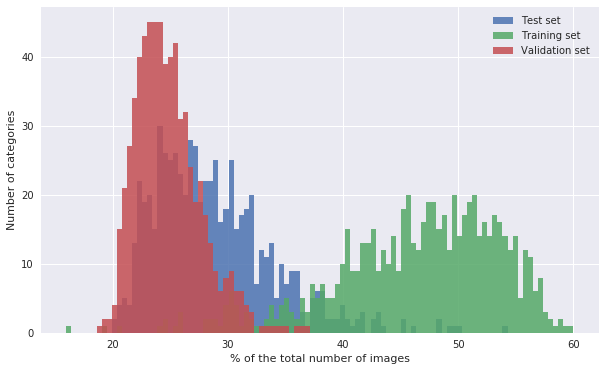
\includegraphics[width=\textwidth]{main/split/split_distribution_trial}
        \caption{Trial experiment dataset splitting method}
        \label{fig:main-split-distribution-trial}
    \end{subfigure}
    \\
    \begin{subfigure}[a]{0.9\textwidth}
        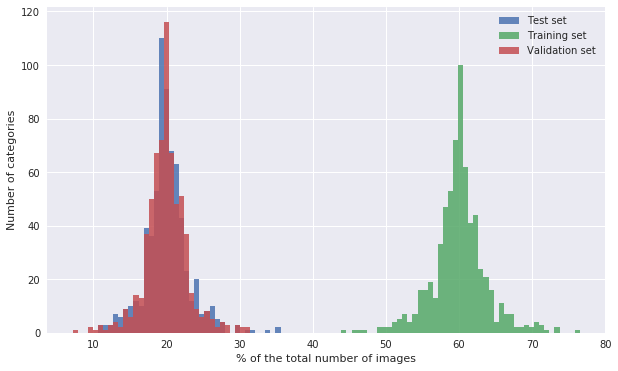
\includegraphics[width=\textwidth]{main/split/split_distribution_main}
        \caption{Main experiment dataset splitting method}
        \label{fig:main-split-distribution-main}
    \end{subfigure}
    \caption{Distribution of the initial image dataset across training, validation and test sets}
    \label{fig:main-split-distribution}
    \end{figure}
    
    The new splitting method was used in all main experiments due to its equal property.
    
\subsection{Classification performance}
    Two pretrained and adapted models were used in the main set of experiments: older and less computational demanding CaffeNet \cite{CaffeNet}, and newer and more advanced GoogleNet \cite{Szegedy2015GoingDeeper}. Both systems were trained to classify 663 selected categories. Achieved classification performance and comparison of these systems are presented in this section
    
    As described in Section \ref{sec:main-training} unlike during the trial set of experiments, a decision on termination of training process during the main set of experiments was based only on the validation loss curve. Specifically, training process was performed until validation loss was stabilized.
    
    Training and validation loss curves for CaffeNet based system is shown on Figure \ref{fig:main-caffenet-training-curve}. Snapshot of the system at 2500 iteration was used for all next computations since while training loss continued to go down being optimized by the solver algorithm, the validation loss remained almost the same in further iterations. In other words, after 2500 iterations the model started to overfit on the training set.
    
    \begin{figure}[H]
        \centering
        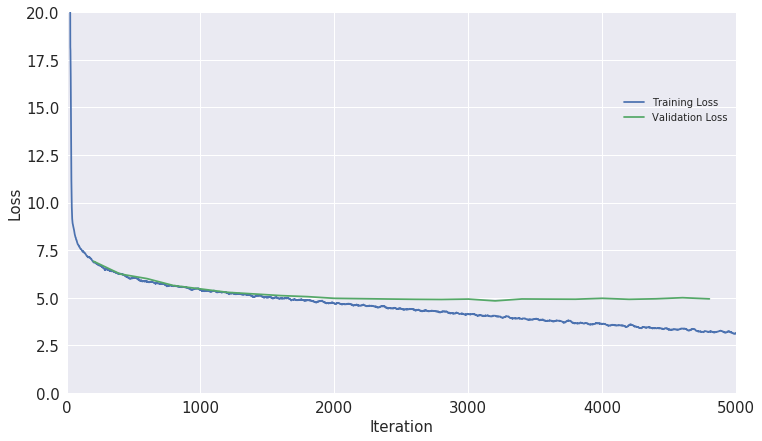
\includegraphics[width=\textwidth]{main/caffenet_training_curve}
        \caption{Training and validation loss curve for CaffeNet based model}
        \label{fig:main-caffenet-training-curve}
    \end{figure}
    
    The same approach was used to determine termination point for GoogleNet model, therefore system snapshot at 35000 iteration was chosen as the most optimal one for the same reasons. Training and validation losses for GoogleNet model are shown on Figure \ref{fig:main-googlenet-training-curve}.
    
    \begin{figure}[H]
        \centering
        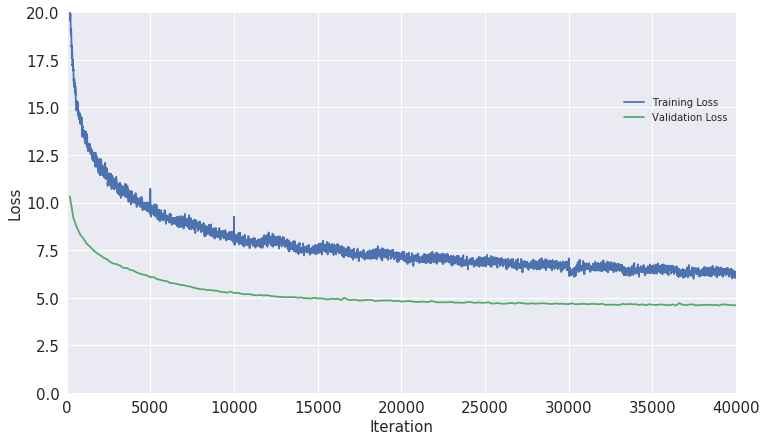
\includegraphics[width=\textwidth]{main/googlenet_training_curve}
        \caption{Training and validation loss curve for GoogleNet based model}
        \label{fig:main-googlenet-training-curve}
    \end{figure}
    
    There is a noticeable difference in the behavior of two training loss curves. It is visually clear that CaffeNet training loss is more stable than the GoogleNet one. This is connected with different batch size used for training of these to networks. As it was mentioned in Methods chapter, due to the bigger number of layers in GoogleNet than CaffeNet this model also requires more GPU memory to perform training, therefore the number of images that can be processed in one iteration is also smaller (128 images in GoogleNet compared to 900 in CaffeNet case for a given GPU). Since in the setup used, the solver optimizes network weights based on a single iteration, smaller number of images lead to less generalizable changes in weights for the whole dataset. As a result, the difference in training loss between two iterations can be bigger.
    
    It is hard to show classification performance for each category due to the big number of them. Therefore several charts were built in order to give insights on the general level of average precision of trained classification systems. Average precision values for the top 40 categories of CaffeNet system are compared with values for the same categories from the GoogleNet model on Figure \ref{fig:main-ap-top-40}. GoogleNet has better average precision in 26 (65\%) of these categories. The same top 5 categories (\textit{football}, \textit{skiing}, \textit{alone}, \textit{icehockey}, and \textit{team-handball}), in an identical order appear in both implementations. Similar to the trial set of experiments, sports categories were highly represented in the top categories for both CaffeNet and GoogleNet systems. 36 out of 40 categories have more than 400 images in the training sample. Specifically, the mean value for the size of the training sample for these categories is 22848.85 with the standard deviation of 47529.22.
    
    The same comparison, but for the bottom 40 CaffeNet categories is shown on Figure \ref{fig:main-ap-bottom-40}. There is a much bigger deviation in values between two implementations than on the previous chart. Out of the 40 categories, 38 contain less than 400 images in the training sample. The mean value for the size of the training sample for these categories is 409.52 with the standard deviation of 222.55.  %This can be connected to the fact that all of these categories, except \textit{laughter} and \textit{grimaces}, contained less than 400 images in the training sample. Therefore for these categories end system performance can be more sensitive to a small changes in the weights.
    
    
    \begin{figure}[H]
        \centering
        \begin{subfigure}[a]{0.95\textwidth}
            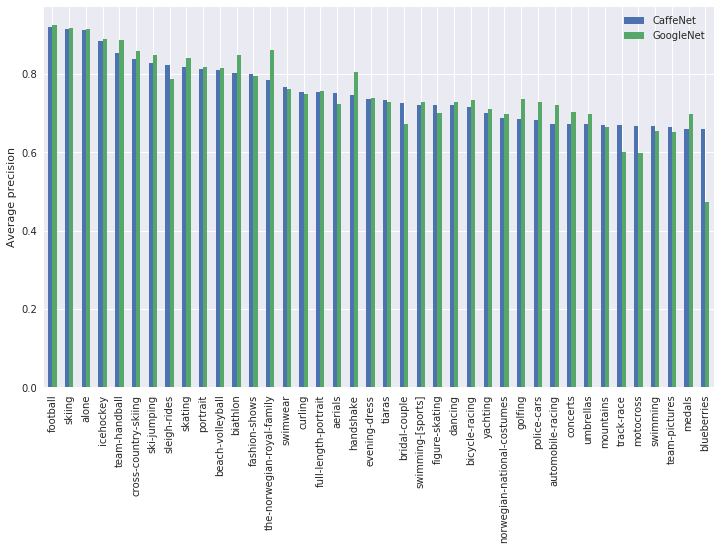
\includegraphics[width=\textwidth]{main/ap_top_40}
            \caption{Top 40 categories}
            \label{fig:main-ap-top-40}
        \end{subfigure}
        \\
        \begin{subfigure}[a]{0.95\textwidth}
            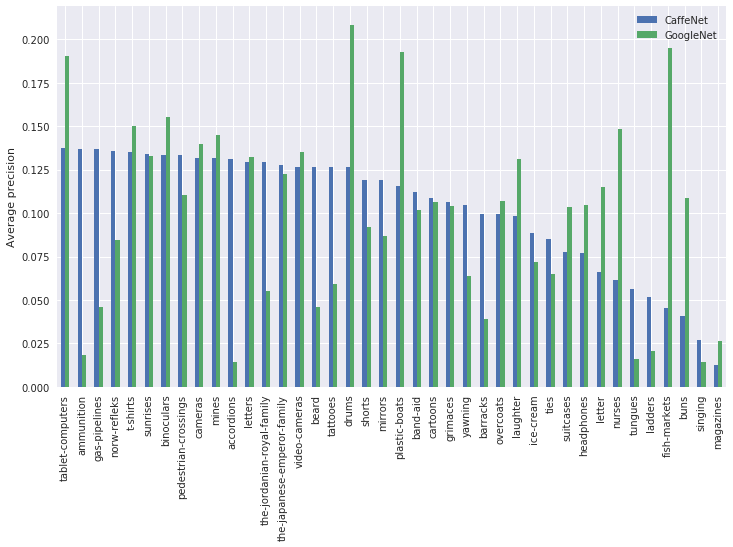
\includegraphics[width=\textwidth]{main/ap_bottom_40}
            \caption{Bottom 40 categories}
            \label{fig:main-ap-bottom-40}
        \end{subfigure}
        \caption{Comparison of average precision results for best and worst categories for main experiment (sorted by CaffeNet values)}
        \label{fig:main-ap}
    \end{figure}
    
    To compare performance for all categories the distribution of the categories across the series of average precision values is shown on Figure \ref{fig:main-ap-dist}. The distribution for both systems covers almost the entire range of precision values. The GoogleNet based system have more categories in both the lower and higher ends of the precision scale. The whole distribution of this system is also more shifted towards the lower values, while CaffeNet based one is concentrated in the middle part of the range. The mean average precision value for the CaffeNet based system was 0.375 with the standard deviation of 0.173, for the system based on the GoogleNet the mean average precision value was 0.34 with the standard deviation of 0.184.
    
    \begin{figure}[H]
        \centering
        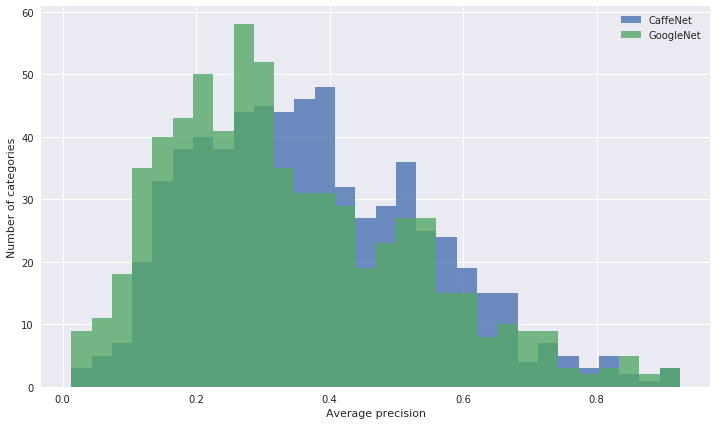
\includegraphics[width=\textwidth]{main/ap_dist}
        \caption{Comparison of CaffeNet and GoogleNet average precision distribution for the main experiment}
        \label{fig:main-ap-dist}
    \end{figure}
    
    The charts showed on Figure \ref{fig:main-ap-vs-size} give insights on how average precision is dependent on the sample size for both systems. While the first chart on Figure \ref{fig:main-ap-vs-size-linear} has linear scale of horizontal axes, the second one on Figure \ref{fig:main-ap-vs-size-log} has logarithmic scale on the size axes. The logarithmic curve of the first chart, as well as linear nature of the second chart, imply the logarithmic dependency between two parameters, which confirms similar observations made during trial experiments. Until particular limit, the small increase in the sample size for a category can give a big increase in the resulting average precision. After reaching the limit, the behavior is opposite -- a big increase in the sample size result in a small increase of the end precision. The second chart also reveals a big difference in the average precision for the categories with similar sample sizes, which was also the case in the trial set of experiments. Confirming observations from the previous charts, GoogleNet based system is concentrated in the lower range of the average precision for categories with a small number of sample images, while CaffeNet based system has more categories within the middle range of average precision values.
    
    \begin{figure}[H]
        \centering
        \begin{subfigure}[a]{\textwidth}
            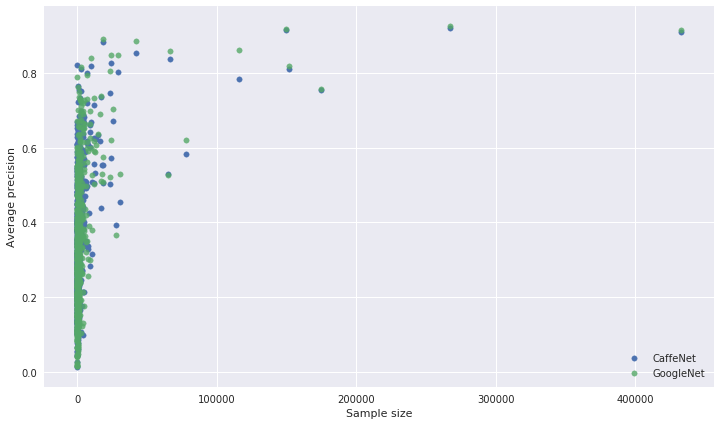
\includegraphics[width=\textwidth]{main/ap_vs_size_linear}
            \caption{Linear scale on horizontal axes}
            \label{fig:main-ap-vs-size-linear}
        \end{subfigure}
        \\
        \begin{subfigure}[a]{\textwidth}
            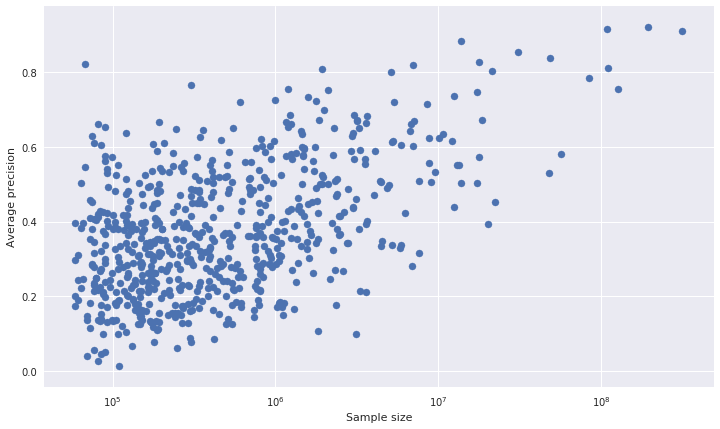
\includegraphics[width=\textwidth]{main/ap_vs_size_log}
            \caption{Logarithmic scale on horizontal axes}
            \label{fig:main-ap-vs-size-log}
        \end{subfigure}
        \caption{Comparison of CaffeNet and GoogleNet average precision vs category sample size for the main experiment}
        \label{fig:main-ap-vs-size}
    \end{figure}
    
    Examples of precision-recall curves for the three categories, \textit{football}, \textit{the-norwegian-royal-family}, and \textit{distance-running}, are given on Figure \ref{main-pr}. The \textit{football category} was category with the best average precision value for both implementations. However, GoogleNet based system has slightly higher average precision for this category, which is also represented on Figure \ref{fig:main-pr-football} where its precision drops at a higher value of the recall level. The same pattern repeats for \textit{the-norwegian-royal-family} category on Figure \ref{fig:main-pr-royal}. The opposite case is for \textit{distance-running} category where CaffeNet implementation have higher precision values almost within entire recall range.
    
    \begin{figure}[h!]
        \centering
        \begin{subfigure}[a]{0.8\textwidth}
            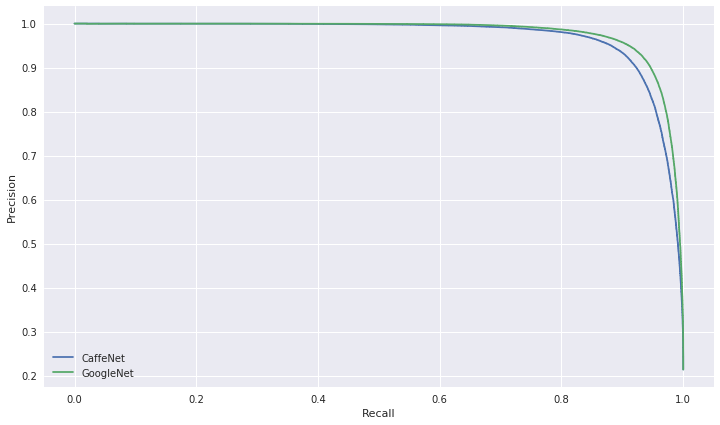
\includegraphics[width=\textwidth]{main/pr_football}
            \caption{Precision-recall curve for \textit{football} category}
            \label{fig:main-pr-football}
        \end{subfigure}
        \\
        \begin{subfigure}[a]{0.8\textwidth}
            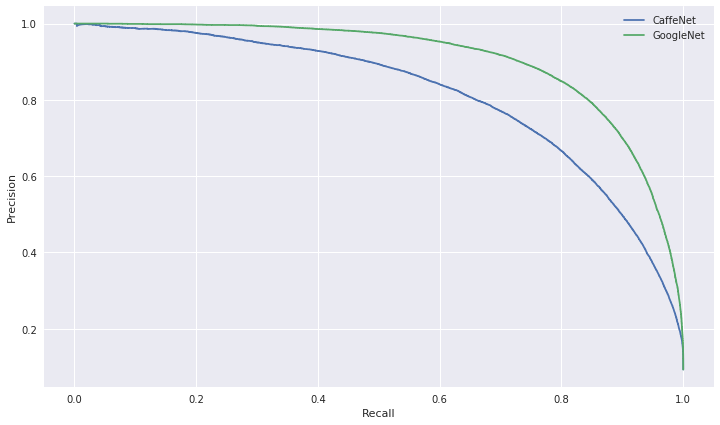
\includegraphics[width=\textwidth]{main/pr_norw_royal}
            \caption{Precision-recall curve for \textit{the-norwegian-royal-family} category}
            \label{fig:main-pr-royal}
        \end{subfigure}
        \\
        \begin{subfigure}[a]{0.8\textwidth}
            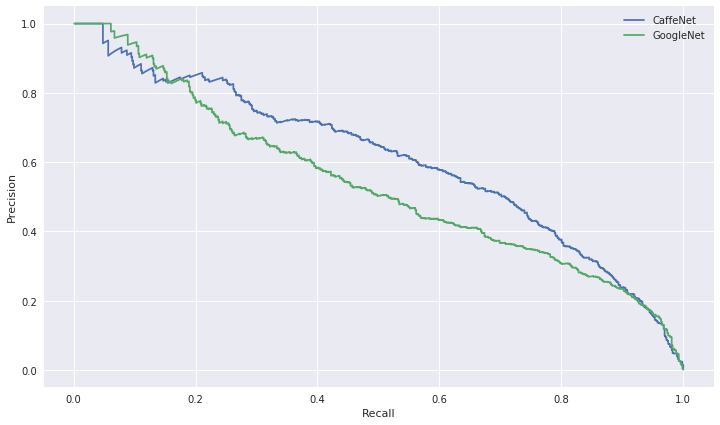
\includegraphics[width=\textwidth]{main/pr_distance_running}
            \caption{Precision-recall curve for \textit{distance-running} category}
            \label{fig:main-pr-distance-running}
        \end{subfigure}
        \caption{Comparison of CaffeNet and GoogleNet precision-recall curves for two categories in main experiment}
        \label{main-pr}
    \end{figure}
    
    It should be mentioned, that the actual system classification performance can be better than indicated by results from this section. The reason for that is a big amount of errors and inconsistency in the initial dataset described earlier. For instance, images that were correctly classified as \textit{full-length-portrait} by GoogleNet based system but did not have this label in the NTB dataset are shown on Figure \ref{fig:main-wrong-flp}. Another example is the pictures shown on Figure \ref{fig:main-wrong-sot} which were classified as \textit{sign-of-triumph} by the system, but did not have the corresponding label in the NTB dataset. Since the NTB dataset was considered as a ground truth in all experiments, such cases were treated as errors of the classification system and lead to reduced average precision results for specific categories. In addition, false negatives errors for some categories were investigated in order to get better understanding of the reasons of the achieved classification performance. This investigation confirmed the hypotesis about negative influence of the contextual images on the average precision results. For example, from 279 images that were labeled as \textit{automobile-racing} in the ground truth set but were not correctly classified to this category by the system 50 (17.9\%) images were also part of the \textit{portrait} or \textit{full-length-portrait} category, 29 (10.4\%) images were part of the \textit{spectators} category, and 22 images were part of the \textit{press-conferences} category; 96 (34.4\%) of images in total were part of at least one of these categories.
    
    \begin{figure}[h!]
        \centering
        \begin{subfigure}[a]{0.31\textwidth}
            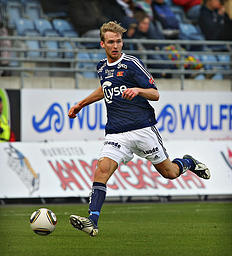
\includegraphics[width=\textwidth]{images/full-length-portrait/sxf48911}
            \caption{Photo by Alf Ove Hansen~/~Scanpix}
        \end{subfigure}
        ~
        \begin{subfigure}[a]{0.31\textwidth}
            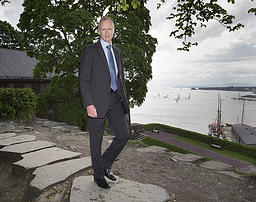
\includegraphics[width=\textwidth]{images/full-length-portrait/sz3bd396}
            \caption{Photo by Terje Bendiksby~/~NTB~scanpix}
        \end{subfigure}
        \\
        \begin{subfigure}[a]{0.31\textwidth}
            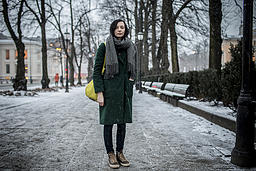
\includegraphics[width=\textwidth]{images/full-length-portrait/sz9fde33}
            \caption{Photo by Stian Lysberg Solum~/~NTB~scanpix}
        \end{subfigure}
        ~
        \begin{subfigure}[a]{0.31\textwidth}
            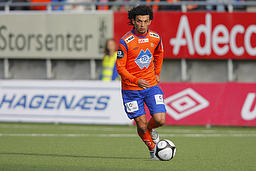
\includegraphics[width=\textwidth]{images/full-length-portrait/sy6a0659}
            \caption{Photo by Svein Ove Ekornesvåg~/~Scanpix}
        \end{subfigure}
        \caption{Examples of images classified as \textit{full-length-portrait}, which were not labeled as such in the NTB database}
        \label{fig:main-wrong-flp}
    \end{figure}
    
    \begin{figure}[h!]
        \centering
        \begin{subfigure}[a]{0.31\textwidth}
            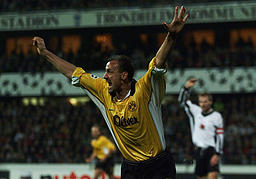
\includegraphics[width=\textwidth]{images/sign-of-triumph/sp02f04c}
            \caption{Photo by Cornelius Poppe~/~Scanpix}
        \end{subfigure}
        ~
        \begin{subfigure}[a]{0.31\textwidth}
            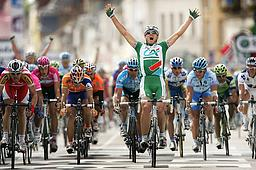
\includegraphics[width=\textwidth]{images/sign-of-triumph/sx281662}
            \caption{Photo by Heiko Junge~/~Scanpix}
        \end{subfigure}
        \\
        \begin{subfigure}[a]{0.31\textwidth}
            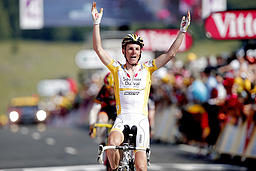
\includegraphics[width=\textwidth]{images/sign-of-triumph/sx6e4b3b}
            \caption{Photo by Stian Lysberg Solum~/~Scanpix}
        \end{subfigure}
        ~
        \begin{subfigure}[a]{0.31\textwidth}
            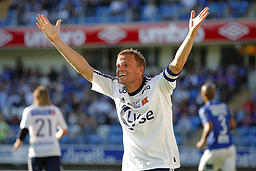
\includegraphics[width=\textwidth]{images/sign-of-triumph/sy1fa403}
            \caption{Photo by Svein Ove Ekornesvåg~/~Scanpix}
        \end{subfigure}
        \caption{Examples of images classified as \textit{sign-of-triumph}, which were not labeled as such in the NTB database}
        \label{fig:main-wrong-sot}
    \end{figure}